\documentclass[10pt,ignorenonframetext,mathserif]{beamer}
\setbeamertemplate{caption}[numbered]
\setbeamertemplate{caption label separator}{: }
\setbeamercolor{caption name}{fg=normal text.fg}
\beamertemplatenavigationsymbolsempty
\usepackage{lmodern}
\usepackage{amssymb,amsmath}
\usepackage{ifxetex,ifluatex}
\usepackage{fixltx2e} % provides \textsubscript
\ifnum 0\ifxetex 1\fi\ifluatex 1\fi=0 % if pdftex
  \usepackage[T1]{fontenc}
  \usepackage[utf8]{inputenc}
\else % if luatex or xelatex
  \ifxetex
    \usepackage{mathspec}
  \else
    \usepackage{fontspec}
  \fi
  \defaultfontfeatures{Ligatures=TeX,Scale=MatchLowercase}
\fi
% use upquote if available, for straight quotes in verbatim environments
\IfFileExists{upquote.sty}{\usepackage{upquote}}{}
% use microtype if available
\IfFileExists{microtype.sty}{%
\usepackage{microtype}
\UseMicrotypeSet[protrusion]{basicmath} % disable protrusion for tt fonts
}{}
\newif\ifbibliography
\hypersetup{
            pdftitle={Useful Skew Design Flow: How To?},
            pdfauthor={Wai-Shing Luk},
            pdfborder={0 0 0},
            breaklinks=true}
\urlstyle{same}  % don't use monospace font for urls
\usepackage{color}
\usepackage{fancyvrb}
\newcommand{\VerbBar}{|}
\newcommand{\VERB}{\Verb[commandchars=\\\{\}]}
\DefineVerbatimEnvironment{Highlighting}{Verbatim}{commandchars=\\\{\}}
% Add ',fontsize=\small' for more characters per line
\newenvironment{Shaded}{}{}
\newcommand{\KeywordTok}[1]{\textcolor[rgb]{0.00,0.44,0.13}{\textbf{#1}}}
\newcommand{\DataTypeTok}[1]{\textcolor[rgb]{0.56,0.13,0.00}{#1}}
\newcommand{\DecValTok}[1]{\textcolor[rgb]{0.25,0.63,0.44}{#1}}
\newcommand{\BaseNTok}[1]{\textcolor[rgb]{0.25,0.63,0.44}{#1}}
\newcommand{\FloatTok}[1]{\textcolor[rgb]{0.25,0.63,0.44}{#1}}
\newcommand{\ConstantTok}[1]{\textcolor[rgb]{0.53,0.00,0.00}{#1}}
\newcommand{\CharTok}[1]{\textcolor[rgb]{0.25,0.44,0.63}{#1}}
\newcommand{\SpecialCharTok}[1]{\textcolor[rgb]{0.25,0.44,0.63}{#1}}
\newcommand{\StringTok}[1]{\textcolor[rgb]{0.25,0.44,0.63}{#1}}
\newcommand{\VerbatimStringTok}[1]{\textcolor[rgb]{0.25,0.44,0.63}{#1}}
\newcommand{\SpecialStringTok}[1]{\textcolor[rgb]{0.73,0.40,0.53}{#1}}
\newcommand{\ImportTok}[1]{#1}
\newcommand{\CommentTok}[1]{\textcolor[rgb]{0.38,0.63,0.69}{\textit{#1}}}
\newcommand{\DocumentationTok}[1]{\textcolor[rgb]{0.73,0.13,0.13}{\textit{#1}}}
\newcommand{\AnnotationTok}[1]{\textcolor[rgb]{0.38,0.63,0.69}{\textbf{\textit{#1}}}}
\newcommand{\CommentVarTok}[1]{\textcolor[rgb]{0.38,0.63,0.69}{\textbf{\textit{#1}}}}
\newcommand{\OtherTok}[1]{\textcolor[rgb]{0.00,0.44,0.13}{#1}}
\newcommand{\FunctionTok}[1]{\textcolor[rgb]{0.02,0.16,0.49}{#1}}
\newcommand{\VariableTok}[1]{\textcolor[rgb]{0.10,0.09,0.49}{#1}}
\newcommand{\ControlFlowTok}[1]{\textcolor[rgb]{0.00,0.44,0.13}{\textbf{#1}}}
\newcommand{\OperatorTok}[1]{\textcolor[rgb]{0.40,0.40,0.40}{#1}}
\newcommand{\BuiltInTok}[1]{#1}
\newcommand{\ExtensionTok}[1]{#1}
\newcommand{\PreprocessorTok}[1]{\textcolor[rgb]{0.74,0.48,0.00}{#1}}
\newcommand{\AttributeTok}[1]{\textcolor[rgb]{0.49,0.56,0.16}{#1}}
\newcommand{\RegionMarkerTok}[1]{#1}
\newcommand{\InformationTok}[1]{\textcolor[rgb]{0.38,0.63,0.69}{\textbf{\textit{#1}}}}
\newcommand{\WarningTok}[1]{\textcolor[rgb]{0.38,0.63,0.69}{\textbf{\textit{#1}}}}
\newcommand{\AlertTok}[1]{\textcolor[rgb]{1.00,0.00,0.00}{\textbf{#1}}}
\newcommand{\ErrorTok}[1]{\textcolor[rgb]{1.00,0.00,0.00}{\textbf{#1}}}
\newcommand{\NormalTok}[1]{#1}
\usepackage{graphicx,grffile}
\makeatletter
\def\maxwidth{\ifdim\Gin@nat@width>\linewidth\linewidth\else\Gin@nat@width\fi}
\def\maxheight{\ifdim\Gin@nat@height>\textheight0.8\textheight\else\Gin@nat@height\fi}
\makeatother
% Scale images if necessary, so that they will not overflow the page
% margins by default, and it is still possible to overwrite the defaults
% using explicit options in \includegraphics[width, height, ...]{}
\setkeys{Gin}{width=\maxwidth,height=\maxheight,keepaspectratio}

% Prevent slide breaks in the middle of a paragraph:
\widowpenalties 1 10000
\raggedbottom

\AtBeginPart{
  \let\insertpartnumber\relax
  \let\partname\relax
  \frame{\partpage}
}
\AtBeginSection{
  \ifbibliography
  \else
    \let\insertsectionnumber\relax
    \let\sectionname\relax
    \frame{\sectionpage}
  \fi
}
\AtBeginSubsection{
  \let\insertsubsectionnumber\relax
  \let\subsectionname\relax
  \frame{\subsectionpage}
}

\setlength{\parindent}{0pt}
\setlength{\parskip}{6pt plus 2pt minus 1pt}
\setlength{\emergencystretch}{3em}  % prevent overfull lines
\providecommand{\tightlist}{%
  \setlength{\itemsep}{0pt}\setlength{\parskip}{0pt}}
\setcounter{secnumdepth}{0}
\usetheme{Rochester}
\setbeamercolor{math text}{fg=purple}
\ifxetex \usepackage[UTF8]{ctex} \fi
\usepackage[footnotesize]{subfigure}
\usepackage{tikz,pgf,pgfplots}
\usetikzlibrary{arrows}
\definecolor{qqqqff}{rgb}{0.,0.,1.}
\newcommand{\columnsbegin}{\begin{columns}}
\newcommand{\columnsend}{\end{columns}}
\newcommand{\col}[1]{\column{#1}}
\pgfdeclareimage[height=0.5cm]{fudan-logo}{fudan-logo.jpg}
\logo{\pgfuseimage{fudan-logo}}

\title{Useful Skew Design Flow: How To?}
\author{Wai-Shing Luk}
\institute{Fudan University}
\date{2017-11-16}

\begin{document}
\frame{\titlepage}

\begin{frame}
\tableofcontents[hideallsubsections]
\end{frame}

\begin{frame}{Useful Skew Design: Why vs.~Why Not}

\begin{block}{Why not}

\begin{itemize}
\tightlist
\item
  Need more engineer training.
\item
  Balanced clock-tree is more difficult to build.
\item
  Don't know how to handle process variation, multi-corner multi-mode,
  \ldots{}, etc.
\end{itemize}

\end{block}

\begin{block}{Why}

If you do it correctly,

\begin{itemize}
\tightlist
\item
  spend less time for struggling timing issues.
\item
  obtain better chip performance or yield.
\end{itemize}

\end{block}

\end{frame}

\begin{frame}{Clock Arrival Time vs.~Clock Skew}

\begin{itemize}
\item
  Clock signal runs periodically.
\item
  Thus, absolute clock arrival time \(u_i\) is not so important.
\item
  Instead, the skew \(y_{ij} = u_j - u_i\) is more important in this
  scenario.
\end{itemize}

\end{frame}

\begin{frame}{Useful Skew Design vs.~Zero-Skew Design}

\begin{itemize}
\tightlist
\item
  ``Critical cycle'' instead of ``critical path''.
\item
  ``Negative cycle'' instead of ``negative slack''.
\item
  If there is a negative cycle, it means that there is no positive slack
  solution no matter how to schedule.
\item
  Others are pretty much the same.
\item
  Same design principle:

  \begin{itemize}
  \tightlist
  \item
    Always tackle the most critical one first!
  \end{itemize}
\end{itemize}

\end{frame}

\begin{frame}{Linear Programming vs.~Network Flow Formulation}

\begin{itemize}
\tightlist
\item
  Linear programming formulation

  \begin{itemize}
  \tightlist
  \item
    can handle more complex constraints
  \end{itemize}
\item
  Network flow formulation

  \begin{itemize}
  \tightlist
  \item
    usually more efficient
  \item
    return the most critical cycle as a bonus.
  \item
    can handle quantized buffer delay (???)
  \end{itemize}
\item
  Anyway, timing analysis is much more time-consuming than the
  optimization solving.
\end{itemize}

\end{frame}

\begin{frame}{Target Skew vs.~Actual Skew}

Don't mess up these two concepts:

\begin{itemize}
\tightlist
\item
  Target skew:

  \begin{itemize}
  \tightlist
  \item
    the skew we want to achieve in the scheduling stage.
  \item
    Usually deterministic (we schedule a meeting at 10:00, rather than
    10:00 \(\pm\) 34 minutes, right?)
  \end{itemize}
\item
  Actual skew

  \begin{itemize}
  \tightlist
  \item
    the skew that the clock tree actually generates.
  \item
    Can be formulated as a random variable.
  \end{itemize}
\end{itemize}

\end{frame}

\section{Background Knowledge}\label{background-knowledge}

\begin{frame}{A Simple Case}

To warm up, let us start with a simple case:

\begin{itemize}
\tightlist
\item
  Assume equal path delay variations.
\item
  Single-corner.
\item
  Before a clock tree is built.
\item
  No adjustable delay buffer (ADB).
\end{itemize}

\end{frame}

\begin{frame}{Network}

\begin{block}{Definition (Network)}

A \emph{network} is a collection of finite-dimensional vector spaces of
\emph{nodes} and \emph{edges}/\emph{arcs}:

\begin{itemize}
\tightlist
\item
  \(V = \{v_1, v_2, \cdots, v_N \}\), where \(|V| = N\)
\item
  \(E = \{e_1, e_2, e_3, \cdots, e_M \}\) where \(|E| = M\)
\end{itemize}

which satisfies 2 requirements:

\begin{enumerate}
\def\labelenumi{\arabic{enumi}.}
\tightlist
\item
  The boundary of each edge is comprised of the union of nodes
\item
  The intersection of any edges is either empty or a boundary node of
  both edges.
\end{enumerate}

\end{block}

\end{frame}

\begin{frame}{Example:}

\begin{figure}[h]
\tikzstyle{vertex}=[circle,fill=black!25,minimum size=20pt,inner sep=0pt]
\tikzstyle{selected vertex} = [vertex, fill=red!24]
\tikzstyle{edge} = [draw,thick,->]
\tikzstyle{weight} = [font=\small]

\begin{tikzpicture}[scale=1.5, auto,swap]
    % Draw a 7,11 network
    % First we draw the vertices
    \foreach \pos/\name in { {(0,2)/a}, {(2,1)/b}, {(4,1)/c},
                             {(0,0)/d}, {(3,0)/e}, {(2,-1)/f}, {(4,-1)/g}}
        \node[selected vertex] (\name) at \pos {$\name$};
    % Connect vertices with edges and draw weights
    \foreach \source/ \dest /\weight in {b/a/-7, c/b/8,d/a/5,d/b/9,
                                         e/b/7, e/c/-5,e/d/-15,
                                         f/d/6,f/e/8,
                                         g/e/9,g/f/-11}
        \path[edge] (\source) -- (\dest);

\end{tikzpicture}
\end{figure}

\end{frame}

\begin{frame}{Orientation}

\begin{block}{Definition (Orientation):}

An \emph{orientation} of an edge is an ordering of its boundary node
\((s, t)\), where

\begin{itemize}
\tightlist
\item
  \(s\) is called a source/initial node
\item
  \(t\) is called a target/terminal node
\end{itemize}

\end{block}

\begin{block}{Definition (Coherent):}

Two orientations to be the same is called \emph{coherent}

\end{block}

\end{frame}

\begin{frame}{Node-edge Incidence Matrix}

\begin{block}{Definition (Incidence Matrix):}

A \(N \times M\) matrix \(A^\top\) is a node-edge incidence matrix with
entries:
\(A(i,j) = \begin{cases} +1 & \text{if } e_i \text{ starts at node } v_j \,, \\ -1 & \text{if } e_i \text{ ends at node } v_j \,, \\ 0 & \text{otherwise } \,. \end{cases}\)

\end{block}

\begin{block}{Example:}

\(A^\top = \begin{bmatrix} 0 & -1 & 1 & 1 & 0 \\ 1 & 1 & 0 & -1 & -1 \\ -1 & 0 & -1 & 0 & 1 \end{bmatrix}\)

\end{block}

\end{frame}

\begin{frame}{Timing Constraint}

\begin{itemize}
\tightlist
\item
  Setup time constraint
  \[y_\text{skew}(i,f) \le T_\text{CP} - D_{if} - T_\text{setup} = u_{if}\] While this
  constraint destroyed, cycle time violation (zero clocking) occurs.
\item
  Hold time constraint \[y_\text{skew}(i,f) \ge T_\text{hold} - d_{if} = l_{if}\]
  While this constraint destroyed, race condition (double clocking)
  occurs.
\end{itemize}

\end{frame}

\begin{frame}{Timing Constraint Graph}

\begin{itemize}
\tightlist
\item
  Create a graph (network) by

  \begin{itemize}
  \tightlist
  \item
    replacing the hold time constraint with an \emph{h-edge} with cost
    \(-(T_\text{hold} - d_{ij})\) from \(\text{FF}_i\) to \(\text{FF}_j\), and
  \item
    replacing the setup time constraint with an s-edge with cost
    \(T_\text{CP} - D_{ij} - T_\text{setup}\) from \(\text{FF}_j\) to \(\text{FF}_i\).
  \end{itemize}
\item
  Two sets of constraints stemming from clock skew definition:

  \begin{itemize}
  \tightlist
  \item
    The sum of skews for paths having the same starting and ending
    flip-flop to be the same;
  \item
    The sum of clock skews of all cycles to be zero
  \end{itemize}
\end{itemize}

\end{frame}

\begin{frame}{Timing Constraint Graph (TCG)}

\columnsbegin
\column{.5\textwidth}

\begin{figure}
\centering
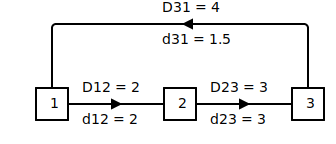
\includegraphics{lec05.files/fig05.png}
\caption{Example circuit}
\end{figure}

\column{.5\textwidth}

\begin{figure}[h!]
\centering
\begin{tikzpicture}[scale=0.8]
\def \radius {2cm}

\node[draw, circle, fill=cyan!20] at ({30}:\radius) (n1) {FF3};
\node[draw, circle, fill=cyan!20] at ({150}:\radius) (n2) {FF1};
\node[draw, circle, fill=cyan!20] at ({270}:\radius) (n3) {FF2};

\path[->, >=latex] (n2) edge [bend left=45] node[above]{CP-4} (n1);
\path[->, >=latex] (n3) edge [bend left=45] node[left]{CP-2} (n2);
\path[->, >=latex] (n1) edge [bend left=45] node[right]{CP-3} (n3);

\path[dashed, ->, >=latex] (n1) edge [bend left=15] node[above]{1.5} (n2);
\path[dashed, ->, >=latex] (n2) edge [bend left=15] node[left]{2} (n3);
\path[dashed, ->, >=latex] (n3) edge [bend left=15] node[right]{3} (n1);

\end{tikzpicture}
\caption{Timing Constraint Graph 
         (Assume $T_\text{setup}$ = $T_\text{hold}$ = 0)}
\end{figure}

\columnsend

\end{frame}

\section{First Thing First}\label{first-thing-first}

\begin{frame}{Meet all timing constraints}

\begin{itemize}
\tightlist
\item
  Find \(y\) in \(\{y \in \mathbb{R}^n \mid y \leq d, A\,u = y\}\)
\item
  How to solve:

  \begin{enumerate}
  \def\labelenumi{\arabic{enumi}.}
  \tightlist
  \item
    Find a negative cycle, fix it.
  \item
    Iterate until no negative cycle is found.
  \end{enumerate}
\item
  Bellman-Ford algorithm (and its variants are publicly available):

  \begin{itemize}
  \tightlist
  \item
    Strongly suggest ``Lazy Evaluation'':

    \begin{itemize}
    \tightlist
    \item
      Don't do full timing analysis on the whole timing graph at the
      beginning!
    \item
      Instead, perform timing analysis only when the algorithm needs.
    \end{itemize}
  \item
    Stop immediately whenever a negative cycle is detected.
  \end{itemize}
\end{itemize}

\end{frame}

\begin{frame}{Delay Padding (DP)}

\begin{itemize}
\tightlist
\item
  Delay padding is a technique that fixes the timing issue by
  intentionally \textbf{solely} ``increasing'' delays.
\item
  Usually formulated as:

  \begin{itemize}
  \tightlist
  \item
    Find \(p, y\) in
    \(\{p, y \in \mathbb{R}^n \mid y \leq d + p, A\,u = y, p \geq 0\}\)
  \end{itemize}
\item
  If the objective is to minimize the sum of \(p\), then the problem is
  the dual of the standard \emph{min-cost flow} problem, which can be
  solved efficiently by the \emph{network simplex} algorithm (publicly
  available).
\item
  Beautiful right?
\end{itemize}

\end{frame}

\begin{frame}{Delay Padding (cont'd)}

\begin{itemize}
\tightlist
\item
  No, the above formulation is not practical.
\item
  In modern design, ``inserting'' a delay may mean swapping a faster
  cell with a slower cell from the cell library. Thus, no need to
  minimize the sum of \(p\).
\item
  More importantly, it may not be possible to find a position to insert
  delay for some delay paths.
\item
  Some papers consider only allowing insert delays to the max-delay path
  only. Some papers consider only allowing insert delays to both the
  max- and min-delay paths together only. None of them are perfect.
\end{itemize}

\end{frame}

\begin{frame}{Delay Padding (cont'd)}

\begin{itemize}
\tightlist
\item
  My suggestion. Instead of calculating the necessary \(p's\) and then
  look for the suitable position to insert, it is easier (and more
  flexible) to determine the position first and then calculate the
  suitable values.
\item
  It can be achieved by modifying the timing graph and solve a
  feasibility problem. Easy enough!
\item
  Quantized delay can be handled too (???).
\end{itemize}

\end{frame}

\begin{frame}{Four possible ways to insert delay}

\begin{figure}[htpb]
\centering
\subfigure[No delay can be inserted]{
\begin{tikzpicture}[scale=0.3]
\def \radius {6cm}
\node[draw, circle, fill=cyan!20] at ({0}:\radius) (n1) {$u_j$};
\node[draw, circle, fill=cyan!20] at ({180}:\radius) (n2) {$u_i$};
\path[->, >=latex] (n2) edge [bend left=35] node[above]{CP-4} (n1);
\path[->, >=latex] (n1) edge [bend left=35] node[above]{1.5} (n2);
\end{tikzpicture}
}
\subfigure[$p_s$, $p_h$ independently]{
\begin{tikzpicture}[scale=0.3]
\def \radius {6cm}
\node[draw, circle, fill=cyan!20] at ({0}:\radius) (n1) {$u_j$};
\node[draw, circle, fill=cyan!20] at ({180}:\radius) (n2) {$u_i$};
\node[draw, circle, fill=red!20] at (0,2) (n3) {$u_s$};
\node[draw, circle, fill=red!20] at (0,-2) (n4) {$u_h$};
\path[->, >=latex] (n3) edge [bend left=-15] node[above]{0} (n2);
\path[->, >=latex] (n3) edge [bend left=15] node[above]{CP-4} (n1);
\path[->, >=latex] (n1) edge [bend left=15] node[above]{1.5} (n4);
\path[->, >=latex] (n4) edge [bend left=15] node[above]{0} (n2);
\end{tikzpicture}
}
\subfigure[$p_s = p_h$]{
\begin{tikzpicture}[scale=0.3]
\def \radius {6cm}
\node[draw, circle, fill=cyan!20] at ({0}:\radius) (n1) {$u_j$};
\node[draw, circle, fill=cyan!20] at ({180}:\radius) (n2) {$u_i$};
\node[draw, circle, fill=red!20] at (0,0) (n3) {$u_k$};
\path[->, >=latex] (n3) edge  node[above]{0} (n2);
\path[->, >=latex] (n3) edge [bend left=35] node[above]{CP-4} (n1);
\path[->, >=latex] (n1) edge [bend left=35] node[above]{1.5} (n3);
\end{tikzpicture}
}
\subfigure[$p_s \geq p_h$]{
\begin{tikzpicture}[scale=0.3]
\def \radius {6cm}
\node[draw, circle, fill=cyan!20] at ({0}:\radius) (n1) {$u_j$};
\node[draw, circle, fill=cyan!20] at ({180}:\radius) (n2) {$u_i$};
\node[draw, circle, fill=red!20] at (0,2) (n3) {$u_s$};
\node[draw, circle, fill=red!20] at (0,-2) (n4) {$u_h$};
\path[->, >=latex] (n3) edge [bend left=-15] node[above]{0} (n2);
\path[->, >=latex] (n3) edge [bend left=15] node[above]{CP-4} (n1);
\path[->, >=latex] (n1) edge [bend left=15] node[above]{1.5} (n4);
\path[->, >=latex] (n4) edge [bend left=15] node[above]{0} (n2);
\path[->, >=latex] (n3) edge [bend left=15] node[right]{0} (n4);
\end{tikzpicture}
}
\caption{}
\end{figure}

\end{frame}

\begin{frame}{Delay Padding (cont'd)}

\begin{itemize}
\tightlist
\item
  If there exists a negative cycle in the modified timing graph, it
  implies that the timing problem cannot be fixed by simply the delay
  padding technique.

  \begin{itemize}
  \tightlist
  \item
    Then, try decrease \(D_{ij}\), or increase \(T_\text{CP}\)
  \end{itemize}
\item
  Be aware of the min-delay path is still the min-delay path after a
  certain amount of delay is inserted (how???).
\end{itemize}

\end{frame}

\section{Variation Issue}\label{variation-issue}

\begin{frame}{Yield-driven Clock Skew Scheduling}

\begin{itemize}
\tightlist
\item
  Assume all timing issues are fixed.
\item
  Now, how to schedule the arrival times to maximize yield?
\item
  According to the critical-first principle, we seek for the most
  critical cycle first.
\item
  The problem can be formulated as:

  \begin{itemize}
  \tightlist
  \item
    \(\max\{\beta \in \mathbb{R} \mid y \leq d - \beta, A\,u = y\}\).
  \end{itemize}
\item
  It is equivalent to the \emph{minimum mean cycle} problem, which can
  be solved efficiently by for example \emph{Howard's algorithm}
  (publicly available).
\end{itemize}

\end{frame}

\begin{frame}{Minimum Balancing Algorithm}

\begin{itemize}
\tightlist
\item
  Then we evenly distribute the slack on this cycle.
\item
  To continue the next most critical cycle, we contract the first one
  into a ``super vertex'' and repeat the process.
\item
  The process stops when the timing graph remains only a single vertex.
\item
  The overall method is known as \emph{minimum balancing} (MB) algorithm
  in the literature.
\end{itemize}

\end{frame}

\begin{frame}{Example: Most timing-critical cycle}

The most vulnerable timing constraint

\begin{tikzpicture}
\def \radius {2cm}

\node[draw, circle, fill=cyan!20] at ({30}:\radius) (n1) {FF3};
\node[draw, circle, fill=cyan!20] at ({150}:\radius) (n2) {FF1};
\node[draw, circle, fill=cyan!20] at ({270}:\radius) (n3) {FF2};

\path[->, >=latex] (n2) edge [bend left=45] node[above]{0.5} (n1);
\path[->, >=latex] (n3) edge [bend left=45] node[left]{2.5} (n2);
\path[->, >=latex] (n1) edge [bend left=45] node[right]{1.5} (n3);

\path[dashed, ->, >=latex] (n1) edge [bend left=15] node[above]{1.5} (n2);
\path[dashed, ->, >=latex] (n2) edge [bend left=15] node[left]{2} (n3);
\path[dashed, ->, >=latex] (n3) edge [bend left=15] node[right]{3} (n1);

\end{tikzpicture}

\end{frame}

\begin{frame}{Example: Distribute the slack}

\begin{itemize}
\tightlist
\item
  Distribute the slack evenly along the most timing-critical cycle.
\end{itemize}

\columnsbegin
\column{.6\textwidth}

\begin{tikzpicture}
\def \radius {2cm}

\node[draw, circle, fill=cyan!20] at ({30}:\radius) (n1) {$T_3$};
\node[draw, circle, fill=cyan!20] at ({150}:\radius) (n2) {$T_1$};
\node[draw, circle, fill=cyan!20] at ({270}:\radius) (n3) {$T_2$};

\path[->, >=latex] (n2) edge [bend left=45] node[above]{0.5} (n1);
\path[->, >=latex] (n3) edge [bend left=45] node[left]{2.5} (n2);
\path[->, >=latex] (n1) edge [bend left=45] node[right]{1.5} (n3);

\path[dashed, ->, >=latex] (n1) edge [bend left=15] node[above]{1.5} (n2);
\path[dashed, ->, >=latex] (n2) edge [bend left=15] node[left]{2} (n3);
\path[dashed, ->, >=latex] (n3) edge [bend left=15] node[right]{3} (n1);

\end{tikzpicture}

\pause
\column{.4\textwidth} \includegraphics{lec05.files/fig10.png}\\
\columnsend

\end{frame}

\begin{frame}{}

\begin{itemize}
\tightlist
\item
  To determine the optimal slacks and skews for the rest of the graph,
  we replace the critical cycle with a super vertex.
\end{itemize}

\columnsbegin
\column{.4\textwidth}

\begin{tikzpicture}
\def \radius {2cm}

\node[draw, circle, fill=cyan!20] at ({30}:\radius) (n1) {0};
\node[draw, circle, fill=cyan!20] at ({150}:\radius) (n2) {0.5};
\node[draw, circle, fill=cyan!20] at ({270}:\radius) (n3) {$T_2$};

\path[->, >=latex, color=red] (n2) edge [bend left=45] node[above]{0.5} (n1);
\path[->, >=latex] (n3) edge [bend left=45] node[left]{2.5} (n2);
\path[->, >=latex] (n1) edge [bend left=45] node[right]{1.5} (n3);

\path[dashed, ->, >=latex, color=red] (n1) edge [bend left=15] node[above]{1.5} (n2);
\path[dashed, ->, >=latex] (n2) edge [bend left=15] node[left]{2} (n3);
\path[dashed, ->, >=latex] (n3) edge [bend left=15] node[right]{3} (n1);

\end{tikzpicture}

\pause
\column{.3\textwidth}

\begin{tikzpicture}
\def \radius {2cm}

\node[draw, rectangle, fill=yellow] at ({90}:\radius) (ns) {\Large{$T_s$}};
\node[draw, circle, fill=cyan!20] at ({270}:\radius) (n3) {$T_2$};

\path[->, >=latex] (n3) edge [bend left=60] node[left]{2} (ns);
\path[->, >=latex] (ns) edge [bend left=60] node[right]{1.5} (n3);

\path[dashed, ->, >=latex] (ns) edge [bend left=25] node[left]{2.5} (n3);
\path[dashed, ->, >=latex] (n3) edge [bend left=25] node[right]{3} (ns);

\end{tikzpicture}

\pause
\column{.3\textwidth} \includegraphics{lec05.files/fig13.png}\\
\columnsend

\end{frame}

\begin{frame}{Repeat the process iteratively}

\columnsbegin
\column{.5\textwidth}

\begin{tikzpicture}
\def \radius {2cm}

\node[draw, rectangle, fill=yellow] at ({90}:\radius) (ns) {\Large{$T_s$}};
\node[draw, circle, fill=cyan!20] at ({270}:\radius) (n3) {$T_2$};

\path[->, >=latex] (n3) edge [bend left=60] node[left]{2} (ns);
\path[->, >=latex] (ns) edge [bend left=60] node[right]{1.5} (n3);

\end{tikzpicture}

\pause
\column{.5\textwidth} \includegraphics{lec05.files/fig15.png}\\
\columnsend

\end{frame}

\begin{frame}{Repeat the process iteratively}

\columnsbegin
\column{.5\textwidth}

\begin{tikzpicture}
\def \radius {2cm}

\node[draw, rectangle, fill=yellow] at ({90}:\radius) (ns) {\Large{$0.25$}};
\node[draw, circle, fill=cyan!20] at ({270}:\radius) (n3) {$0$};

\path[->, >=latex] (n3) edge [bend left=60] node[left]{2} (ns);
\path[->, >=latex] (ns) edge [bend left=60] node[right]{1.5} (n3);

\end{tikzpicture}

\column{.5\textwidth} \includegraphics{lec05.files/fig15.png}\\
\columnsend

\end{frame}

\begin{frame}{Final result}

\columnsbegin
\column{.5\textwidth}

\begin{itemize}
\item
  Skew\(_{12}\) = 0.75
\item
  Skew\(_{23}\) = -0.25
\item
  Skew\(_{31}\) = -0.5
\item
  Slack\(_{12}\) = 1.75
\item
  Slack\(_{23}\) = 1.75
\item
  Slack\(_{31}\) = 1
\end{itemize}

where Slack\(_{ij}\) = CP - D\(_{ij}\) - T\(_\text{setup}\) -
Skew\(_{ij}\)

\column{.5\textwidth}

\begin{tikzpicture}
\def \radius {2cm}

\node[draw, circle, fill=cyan!20] at ({30}:\radius) (n1) {0.25};
\node[draw, circle, fill=cyan!20] at ({150}:\radius) (n2) {0.75};
\node[draw, circle, fill=cyan!20] at ({270}:\radius) (n3) {0};

\path[->, >=latex] (n2) edge [bend left=45] node[above]{0.5} (n1);
\path[->, >=latex] (n3) edge [bend left=45] node[left]{2.5} (n2);
\path[->, >=latex] (n1) edge [bend left=45] node[right]{1.5} (n3);

\path[dashed, ->, >=latex] (n1) edge [bend left=15] node[above]{1.5} (n2);
\path[dashed, ->, >=latex] (n2) edge [bend left=15] node[left]{2} (n3);
\path[dashed, ->, >=latex] (n3) edge [bend left=15] node[right]{3} (n1);

\end{tikzpicture}

\columnsend

\end{frame}

\begin{frame}{What the MB algorithm really give us?}

\begin{itemize}
\tightlist
\item
  The MB algorithm not only give us the scheduling solution, but also a
  tree-topology that represents the order of ``criticality''!
\end{itemize}

\begin{figure}
\centering
\begin{tikzpicture}[sibling distance=5em,
  every node/.style = {shape=rectangle, rounded corners,
    draw, align=center,
    top color=white, bottom color=blue!20}]
  \node {$T_{s3}$}
    child { node {$T_5$} }
    child { node {$T_{s1}$ }
      child { node {$T_1$} }
      child { node {$T_2$} } }
    child { node {$T_6$} }
    child { node {$T_{s2}$ }
      child { node {$T_3$} }
      child { node {$T_4$} } };
\end{tikzpicture}
\end{figure}

\end{frame}

\begin{frame}{Clock-tree Synthesis and Placement}

\begin{itemize}
\tightlist
\item
  I strongly suggest that the topology of the clock-tree precisely
  follows the order of ``criticality''!

  \begin{itemize}
  \tightlist
  \item
    since the lower branch of clock-tree has smaller skew variation.
  \end{itemize}
\item
  I also suggest that the placer should follow the topology of the
  clock-tree:

  \begin{itemize}
  \tightlist
  \item
    Physically place the registers of the same branch together.
  \item
    The locality implies stronger correlation of variations and implies
    even smaller skew variation due to the cancellation effect.
  \item
    Note that the current SSTA does not provide the correlation
    information, so this is the best you can do!
  \end{itemize}
\end{itemize}

\end{frame}

\begin{frame}{Second Example: Yield-driven Clock Skew Scheduling}

\begin{itemize}
\tightlist
\item
  Now assume that SSTA (or STA+OCV, POCV, AOCV) is performed.
\item
  Let (\(\bar{d}\), \(s\)) be the (mean, variance) of \(\mathbf{d}\)
\item
  The most critical cycle can be obtained by solving:

  \begin{itemize}
  \tightlist
  \item
    \(\max\{\beta \in \mathbb{R} \mid y \leq \bar{d} - \beta s, A\,u = y\}\)
  \end{itemize}
\item
  It is equivalent to the minimum cost-to-time ratio cycle problem,
  which can be solved efficiently by for example Howard's algorithm
  (publicly available).
\item
  Gaussian distribution is assumed. For arbitary distribution, see my
  DAC'08 paper.
\end{itemize}

\end{frame}

\begin{frame}{What About the Correlation?}

\begin{itemize}
\tightlist
\item
  In the above formulation, we minimum the maximum possibility of timing
  violation of each \emph{individual} timing constraint. So only
  individual delay distribution is needed.
\item
  Yes, the objective function is not the true timing-yield. But it is
  reasonable, easy to solve, and is the best you can do so far.
\end{itemize}

\end{frame}

\section{Multi-Corner Issue}\label{multi-corner-issue}

\begin{frame}{Meet all timing constraints in Multi-Corner:}

\begin{itemize}
\tightlist
\item
  Assume no Adjustable Delay Buffer (ADB)
\item
  Find \(y\) in
  \(\{y \in \mathbb{R}^n \mid y \leq d^{(k)}, A\,u = y, \forall k\in[1..K]\}\)
\item
  Equivalent to finding \(y\) in
  \(\{y \in \mathbb{R}^n \mid y \leq \min_k\{ d^{(k)}\}, A\,u = y \}\)
\item
  Feasibility problem
\item
  How to solve:

  \begin{enumerate}
  \def\labelenumi{\arabic{enumi}.}
  \tightlist
  \item
    Find a negative cycle, fix it.
  \item
    Iterate until no negative cycle is found.
  \end{enumerate}
\item
  Better avoid fixing the timing issue corner-by-corner. Inducing
  ping-pong effect.
\end{itemize}

\end{frame}

\begin{frame}{Delay padding (DP) in Multi-Corner}

\begin{itemize}
\tightlist
\item
  The problem CANNOT be formulated as a network flow problem. But still
  you can solve it by a linear programming formulation.
\item
  Or, decomposite the problem into subproblems for each corner.
\item
  Again use the modified timing graph technique.
\item
  Then, \(y\)'s are shared variables of subproblems.
\item
  If we solve each subproblem individually, the solution will not agree
  with each other. Induce \emph{ping-pong effect}.
\item
  Need something to drive the agreement.
\end{itemize}

\end{frame}

\begin{frame}{Delay Padding (DP) in Multi-Corner (cont'd)}

\begin{itemize}
\tightlist
\item
  Follow the idea of \emph{dual decomposition}: If a solution is above
  the average. then introduce a punishment cost. If a solution is below
  the average, then introduce a rewarding cost.
\item
  Then, each subproblem is a min-cost potential problem, which can be
  solved efficiently.
\item
  If some subproblems do not have feasible solutions, it implies that
  the problem cannot be fixed by simply delay padding.
\item
  The process repeats until all solutions converge. If not, it implies
  that the problem cannot be fixed by simply delay padding.
\end{itemize}

\end{frame}

\begin{frame}{Yield-driven Clock Skew Scheduling:}

\begin{itemize}
\tightlist
\item
  \(\max\{\beta \in \mathbb{R} \mid y \leq d^{(k)} - \beta s, A\,u = y, \forall k\in[1..K]\}\)
\item
  More or less the same as in Single Corner.
\end{itemize}

\end{frame}

\section{Clock-Tree Issue}\label{clock-tree-issue}

\begin{frame}{Clock Tree Synthesis (CTS)}

\begin{itemize}
\tightlist
\item
  Construct merging location

  \begin{itemize}
  \tightlist
  \item
    DME algorithm, Elmore delay, buffer insertion
  \end{itemize}
\item
  Some research on \emph{bounded-skew DME algorithm}. But the algorithm
  is too complicated in my opinion.
\item
  If the previous stage is over-optimized, the clock tree is hard to
  implement. If it happens, some budgeting techniques should be invoked
  (engineering issue)
\item
  After a clock tree is constructed, more accurate timing (rather than
  Elmore delay) can be obtained via timing analysis.
\end{itemize}

\end{frame}

\begin{frame}{Co-optimization Issue}

\begin{itemize}
\tightlist
\item
  After a clock tree is built, we have a clearer picture.
\item
  Should I perform the re-scheduling? And how?
\item
  Some papers suggest adding a factor to the timing constraint, say:
  \[1.2 u_i - 0.8 u_j \leq w_{ij}\].
\item
  Then the formulation is not a kind of network-flow, but may still be
  solvable by linear programming.
\item
  Need to investigate more deeply.
\end{itemize}

\end{frame}

\section{Adjustable Delay Buffer
Issue}\label{adjustable-delay-buffer-issue}

\begin{frame}{Adjustable delay buffers in Multi-Mode}

\begin{itemize}
\tightlist
\item
  Assume adjustable delay buffers are added solely to the clock tree
\item
  Hence, each mode can have a different set of arrival times.
\item
  Easier for clock skew scheduling, harder for clock-tree synthesis.
\end{itemize}

\end{frame}

\begin{frame}{Meet timing constraint in Multi-Mode:}

\begin{itemize}
\tightlist
\item
  find \(y^{(m)}\) in
  \(\{y^{(m)} \in \mathbb{R}^n \mid y^{(m)} \leq d^{(m)}, A\,u^{(m)} = y^{(m)}, \forall m\in[1..M]\}\)
\item
  Can be done in parallel.
\item
  find a negative cycle, fix it (do not need to know all \(d_i^{(m)}\)
  at the beginning) for every mode in parallel.
\end{itemize}

\end{frame}

\begin{frame}{Delay Padding (DP) in Multi-mode}

\begin{itemize}
\tightlist
\item
  Again use a modified timing graph technique.
\item
  NOT a network flow problem. Use LP, or
\item
  Dual decomposition -\textgreater{} min-cost potential problem for each
  mode

  \begin{itemize}
  \tightlist
  \item
    Only \(p\)'s are shared variables.
  \item
    Initial feasible solution obtained by the single-mode method

    \begin{itemize}
    \tightlist
    \item
      A negative cycle =\textgreater{} problem cannot be fixed by DP
    \end{itemize}
  \end{itemize}
\item
  Not converge =\textgreater{} problem cannot be fixed by DP

  \begin{itemize}
  \tightlist
  \item
    Try decrease \(D_{ij}\), or increase \(T_\text{CP}\)
  \end{itemize}
\end{itemize}

\end{frame}

\begin{frame}{Yield-driven Clock Skew Scheduling:}

\begin{itemize}
\tightlist
\item
  \(\max\{\beta \in \mathbb{R} \mid y^{(m)} \leq d^{(m)} - \beta s, A\,u^{(m)} = y^{(m)}, \forall m\in[1..M]\}\)
\item
  Pretty much the same as Single-Mode.
\end{itemize}

\end{frame}

\begin{frame}{Difficulty in ADB Multi-Mode Design}

\begin{itemize}
\tightlist
\item
  How to design the clock-tree?
\item
  What is the order of criticality?
\item
  How to determine the minimum range of ADB?
\end{itemize}

\end{frame}

\begin{frame}{Thank you for your attention!}

\end{frame}

\begin{frame}[fragile]{Backup}

\begin{Shaded}
\begin{Highlighting}[]
\ExtensionTok{pandoc}\NormalTok{ -s -t beamer --toc useful_skew.md beamer.yaml \textbackslash{}}
\NormalTok{       -o useful_skew.pdf}
\end{Highlighting}
\end{Shaded}

\end{frame}

\end{document}
